{\documentclass[11pt,a4paper,titlepage,table]{article}
\usepackage[a4paper]{geometry}
\usepackage[utf8]{inputenc}
\usepackage[english]{babel}
\usepackage{lipsum}

\usepackage{amsmath, amssymb, amsfonts, amsthm, fouriernc}
% mathtools for: Aboxed (put box on last equation in align envirenment)
\usepackage{microtype} %improves the spacing between words and letters

\usepackage{graphicx}
\graphicspath{ {./pics/} {./eps/}}
\usepackage{epsfig}
\usepackage{epstopdf}
\usepackage{colortbl}

%%%%%%%%%%%%%%%%%%%%%%%%%%%%%%%%%%%%%%%%%%%%%%%%%%
%% COLOR DEFINITIONS
%%%%%%%%%%%%%%%%%%%%%%%%%%%%%%%%%%%%%%%%%%%%%%%%%% 
\usepackage{colortbl}
\usepackage[usenames,dvipsnames,svgnames,table]{xcolor}
\usepackage{float}
%%%%%%%%%%%%%%%%%%%%%%%%%%%%%%%%%%%%%%%%%%%%%%%%%%
\definecolor{MyColor1}{HTML}{75A42E}
\definecolor{MyColor2}{HTML}{75A42E}
\definecolor{MyColor3}{HTML}{4D6D1E}
\definecolor{green1}{HTML}{EAF5DB}
\definecolor{green2}{HTML}{C2E193}
\definecolor{maroon}{cmyk}{0,0.87,0.68,0.32}
\newcommand{\textb}{\color{Black} \usefont{OT1}{lmss}{m}{n}}
\newcommand{\blue}{\color{MyColor1} \usefont{OT1}{lmss}{m}{n}}
\newcommand{\blueb}{\color{MyColor1} \usefont{OT1}{lmss}{b}{n}}
\newcommand{\red}{\color{LightCoral} \usefont{OT1}{lmss}{m}{n}}
\newcommand{\green}{\color{Turquoise} \usefont{OT1}{lmss}{m}{n}}
%%%%%%%%%%%%%%%%%%%%%%%%%%%%%%%%%%%%%%%%%%%%%%%%%%

%%%%%%%%%%%%%%%%%%%%%%%%%%%%%%%%%%%%%%%%%%%%%%%%%%
%% FONTS AND COLORS
%%%%%%%%%%%%%%%%%%%%%%%%%%%%%%%%%%%%%%%%%%%%%%%%%%
%    SECTIONS
%%%%%%%%%%%%%%%%%%%%%%%%%%%%%%%%%%%%%%%%%%%%%%%%%%
\usepackage{titlesec}
\usepackage{sectsty}
%%%%%%%%%%%%%%%%%%%%%%%%
%set section/subsections HEADINGS font and color
\sectionfont{\color{MyColor1}}  % sets colour of sections
\subsectionfont{\color{MyColor2}}  % sets colour of sections
\subsubsectionfont{\color{MyColor3}}  % sets colour of sections

%set section enumerator to arabic number (see footnotes markings alternatives)
\renewcommand\thesection{\arabic{section}.} %define sections numbering
\renewcommand\thesubsection{\thesection\arabic{subsection}} %subsec.num.

%define new section style
\newcommand{\mysection}{
	\titleformat{\section} [runin] {\usefont{OT1}{lmss}{b}{n}\color{MyColor1}} 
	{\thesection} {3pt} {} } 

%%%%%%%%%%%%%%%%%%%%%%%%%%%%%%%%%%%%%%%%%%%%%%%%%%
%		CAPTIONS
%%%%%%%%%%%%%%%%%%%%%%%%%%%%%%%%%%%%%%%%%%%%%%%%%%
\usepackage{caption}
\usepackage{subcaption}
%%%%%%%%%%%%%%%%%%%%%%%%
\captionsetup[figure]{labelfont={color=MyColor1}}

\makeatletter
\let\reftagform@=\tagform@
\def\tagform@#1{\maketag@@@{(\ignorespaces\textcolor{red}{#1}\unskip\@@italiccorr)}}
\renewcommand{\eqref}[1]{\textup{\reftagform@{\ref{#1}}}}
\makeatother
\usepackage{hyperref}
\hypersetup{colorlinks=true}

%%%%%%%%%%%%%%%%%%%%%%%%%%%%%%%%%%%%%%%%%%%%%%%%%%
%% PREPARE TITLE
%%%%%%%%%%%%%%%%%%%%%%%%%%%%%%%%%%%%%%%%%%%%%%%%%%
\title{\blue  
	\begin{figure}[h!]
  		\centering
    	\includegraphics[width=1\textwidth]{img/logo3}
	\end{figure}
	\blueb Battle of Origins | Interim Release}
\author{Patrick Misteli, Ruben Kälin, Jacqueline Staub, Gregory Wyss}
\date{\today}
%%%%%%%%%%%%%%%%%%%%%%%%%%%%%%%%%%%%%%%%%%%%%%%%%%

\begin{document}
	\maketitle
	\hypersetup{linkcolor=MyColor1}	
	
	\tableofcontents
	\newpage
	
	%\section{Overview}
	
	%In this document we will give a short overview of our progress for the interim release of our game \textit{Battle of Origins}. We will begin with a listing of our targets for every stage where we will highlight the completed, uncompleted and current targets. Afterwards we will list some of the difficulties we encountered in the programming/design areas graphics, artificial intelligence and game logic. At the end you can find the design revisions we decided for and the reasons for these revisions.
	
	\section{Current Stage}
	
	We have implemented the functional minimum and are nearly done with the low target of our project. The following sections will describe our progress and our difficulties. 
	
	\subsection{Task Distribution}
	See Table \ref{table:taskallocProject}
	\begin{table}[h!]\centering
		\newcounter{taskId}
		\setcounter{taskId}{0}
		\begin{tabular}{r|p{10cm}|p{1.8cm}|c|c}
			\textbf{Task} & \textbf{Description} & \textbf{Who} & \textbf{Hrs} & \textbf{Actual} \\
			
			\hline 
			\cellcolor[gray]{0.8} & \multicolumn{4}{c}{\cellcolor[gray]{0.8} Idea Finding}\\
			
			\hline				
			\rowcolor{green}		
			\stepcounter{taskId}
			\thetaskId . & Brainstorming Design &\centering  All & $5$ & $7$ \\
			
			\hline
			\rowcolor{green}
			\stepcounter{taskId}
			\thetaskId . & Character modeling &\centering Greg, Jacq  & $20$ & $25$\\
			
			\hline 
			\cellcolor[gray]{0.8} & \multicolumn{4}{c}{\cellcolor[gray]{0.8} Assignments}\\
			
			\hline
			\rowcolor{green}
			\stepcounter{taskId}
			\thetaskId . & Project Proposal Draft & \centering  All & $10$ & $10$\\
			
			\hline
			\rowcolor{green}
			\stepcounter{taskId}
			\thetaskId . & Prototype Chapter& \centering  All & $10$ & $10$\\
			
			\hline
			\rowcolor{green}
			\stepcounter{taskId}
			\thetaskId . & Interim Report Chapter & \centering  All & $10$ & $10$\\
			
			\hline
			\stepcounter{taskId}
			\thetaskId . & Alpha Release Chapter & \centering  All & $10$ &\\
			
			\hline
			\stepcounter{taskId}
			\thetaskId . & Playtest Chapter & \centering  All & $10$ &\\
			
			\hline
			\stepcounter{taskId}
			\thetaskId . & Conclusion Chapter & \centering  All & $10$ &\\
			
			\hline
			\stepcounter{taskId}
			\thetaskId . & Demo Video & \centering Patrick & $50$ &\\
			
			\hline 
			\cellcolor[gray]{0.8} & \multicolumn{4}{c}{\cellcolor[gray]{0.8} Presentation and Demos}\\
			
			\hline
			\rowcolor{green}
			\stepcounter{taskId}
			\thetaskId . & Pitch of the Game & \centering  All & $7$ & $7$\\
			
			\hline
			\rowcolor{green}
			\stepcounter{taskId}
			\thetaskId . & Formal Game Proposal & \centering  All & $10$ & $12$\\
			
			\hline
			\rowcolor{green}
			\stepcounter{taskId}
			\thetaskId . & Paper Prototype & \centering  Jacqueline & $5$ & $6$\\
			
			\hline
			\rowcolor{green}
			\stepcounter{taskId}
			\thetaskId . & First Playable Demo & \centering  All & $30$ & $50$\\
			
			\hline
			\rowcolor{green}
			\stepcounter{taskId}
			\thetaskId . & Interim Demo & \centering  All & $50$ & $80$\\
			
			\hline
			\stepcounter{taskId}
			\thetaskId . & Alpha Release Demo & \centering  All & $100$ &\\
			
			\hline
			\stepcounter{taskId}
			\thetaskId . & Play-test presentation & \centering  All & $75$ &\\
			
			\hline
			\stepcounter{taskId}
			\thetaskId . &Final Public Presentation & \centering  All & $40$ &\\
			
		\end{tabular}
		
		\caption{\textit{Task allocation}  Green: Completed}
		\label{table:taskallocProject}	
	\end{table}	
	
	\newpage
		
		\subsection{Project Management}
		See Table \ref{table:taskallocEngineer}
		\begin{table}[h!]\centering
			\begin{tabular}{r|p{10cm}|p{1.8cm}|c|c}
				\textbf{Task} & \textbf{Description} & \textbf{Who} & \textbf{Hrs} & \textbf{Actual} \\
				
				\hline 
				\cellcolor[gray]{0.8} & \multicolumn{4}{c}{\cellcolor[gray]{0.8} Functional Minimum}\\
				
				\hline
				\rowcolor{green}
				\stepcounter{taskId}
				\thetaskId . & Players from two teams running around & \centering  All & $15$ & $15$\\
				
				\hline
				\rowcolor{green}
				\stepcounter{taskId}
				\thetaskId . & Level Design: Overflow flat Map & \centering  All & $15$ & $7$\\
				
				
				\hline
				\rowcolor{green}
				\stepcounter{taskId}
				\thetaskId . & Counting collective hits & \centering  All & $15$ & $8$\\
				
				\hline
				\rowcolor{green}
				\stepcounter{taskId}
				\thetaskId . & Game finishes after 8 min & \centering  All & $15$ &$10$\\
				
				
				\hline
				\rowcolor{green}
				\stepcounter{taskId}
				\thetaskId . & Winner is Team with most hits & \centering  All & $15$ &$14$\\
				
				\hline
				\rowcolor{green}
				\stepcounter{taskId}
				\thetaskId . & AI Controlled Allies/Enemies. & \centering  Ruben & $15$ &$25$\\ 
				
				\hline 
				\cellcolor[gray]{0.8} & \multicolumn{4}{c}{\cellcolor[gray]{0.8} Low Target}\\
				
				\hline
				\rowcolor{yellow}
				\stepcounter{taskId}
				\thetaskId . & Audio: Music + Sound Effects & \centering  Patrick & $15$ & $2$\\
				
				\hline
				\rowcolor{green}
				\stepcounter{taskId}
				\thetaskId . & Physics: Players flying away when hit & \centering  All & $15$ &$10$\\
				
				\hline
				\rowcolor{green}
				\stepcounter{taskId}
				\thetaskId . & Physics: Cooldown before being able to move \& attack & \centering  All & $15$ &$17$\\
				
				\hline
				\rowcolor{green}
				\stepcounter{taskId}
				\thetaskId . & Physics: Immunity cooldown before being vulnerable again & \centering  All & $15$ &$13$\\
				
				\hline
				\rowcolor{green}
				\stepcounter{taskId}
				\thetaskId . & Wonder: Wonder is generated after every 50 collective hits & \centering  All & $15$ &$24$\\
				
				\hline
				\rowcolor{green}
				\stepcounter{taskId}
				\thetaskId . & Wonder: Wonder is (visually) possessed by a human player & \centering  All & $15$ &$10$\\
				
				\hline
				\rowcolor{green}
				\stepcounter{taskId}
				\thetaskId . & Wonder: Wonder can visually be cast & \centering  All & $15$ &$12$\\
				
				
				\hline
				\rowcolor{green}
				\stepcounter{taskId}
				\thetaskId . & Wonder: Wonder converts players & \centering  All & $15$ &$16$\\
				
				\hline
				\rowcolor{yellow}
				\stepcounter{taskId}
				\thetaskId . & Wonder: Converted Human player plays for the other team & \centering  All & $15$ & $5$\\
				
				
				\hline
				\rowcolor{green}
				\stepcounter{taskId}
				\thetaskId . & Winner is the team with the most members & \centering  All & $15$ &$20$\\
				
				\hline
				\rowcolor{green}
				\stepcounter{taskId}
				\thetaskId . & Level Design: Map includes obstacles & \centering  All & $15$ &$7$\\
				
				\hline 
				\cellcolor[gray]{0.8} & \multicolumn{4}{c}{\cellcolor[gray]{0.8} Desired Target}\\

				\hline
				\rowcolor{yellow}
				\stepcounter{taskId}
				\thetaskId . & Characters visually polished to look from same theme & \centering Jacqueline, Gregory & $15$ &\\
				
				\hline
				\rowcolor{yellow}
				\stepcounter{taskId}
				\thetaskId . & Wonder Creation: Creating a wonder by standing together and pressing "commit" & \centering  All & $15$ &\\
				
				\hline
				\rowcolor{white}
				\stepcounter{taskId}
				\thetaskId . & Wonder Creation: Cooldown after releasing "commit" & \centering  All & $15$ &\\
				
				\hline
				\rowcolor{white}
				\stepcounter{taskId}
				\thetaskId . & Wonder Creation: Increased vulnerability during praying and cooldown & \centering  All & $15$ &\\
				
				\hline
				\rowcolor{yellow}
				\stepcounter{taskId}
				\thetaskId . & Wonder Creation: Larger praying/studying circles will generate quicker progress & \centering  All & $15$ &\\
				
				\hline
				\rowcolor{white}
				\stepcounter{taskId}
				\thetaskId . & Wonder Creation: AI upgrade to take wonder creation into account & \centering  All & $15$ &\\			
				
				\hline 
				\rowcolor{white}
				\cellcolor[gray]{0.8} & \multicolumn{4}{c}{\cellcolor[gray]{0.8} High Target}\\
				
				\hline
				\stepcounter{taskId}
				\thetaskId . & Converted Human player will control free NPC if available & \centering  All & $15$ &\\
				
				\hline
				\rowcolor{yellow}
				\stepcounter{taskId}
				\thetaskId . & Players evolve numerically according to their actions (Running, Shooting, Praying/Studying) & \centering  All & $15$ &\\
				
				\hline
				\stepcounter{taskId}
				\thetaskId . & Players evolve visually & \centering  All & $15$ &\\
				
				\end{tabular}
				
				\caption{\textit{Task allocation} Green: Completed, Yellow: in Progress}
				\label{table:taskallocEngineer}	
				\end{table}
				
				\newpage
				
				\subsection{Timeline}
				See Table \ref{table:timeline1} and Table \ref{table:timeline2}
				
				
				\begin{table}[h!]\centering
					\setcounter{taskId}{0}
					\begin{tabular}{r|c|c|c|c|c|c|c|c|c|c|c|c|c|c}
						\textbf{Task} & \textbf{W1} & \textbf{W2} & \textbf{W3} & \textbf{W4} & \textbf{W5} & \textbf{W6} & \textbf{W7} & \textbf{W8} & \textbf{W9} & \textbf{W10} & \textbf{W11} & \textbf{W12} & \textbf{W13} & \textbf{W14}\\
						
						\hline 
						\cellcolor[gray]{0.8} & \multicolumn{14}{c}{\cellcolor[gray]{0.8} Idea Finding}\\
						
						\hline						
						\stepcounter{taskId}
						\thetaskId . & A & A & & & & & & & & & & & & \\
						
						\hline						
						\stepcounter{taskId}
						\thetaskId . & G & G & & & & & & & & & & & & \\
						
						\hline 
						\cellcolor[gray]{0.8} & \multicolumn{14}{c}{\cellcolor[gray]{0.8} Assignments}\\
						
						\hline						
						\stepcounter{taskId}
						\thetaskId . & & A & A & & & & & & & & & & & \\
						
						\hline						
						\stepcounter{taskId}
						\thetaskId . & & & & J & A & & & & & & & & & \\
						
						\hline						
						\stepcounter{taskId}
						\thetaskId . & & & & & & A & A & A & A & & & & & \\
						
						\hline						
						\stepcounter{taskId}
						\thetaskId . & & & & & & & & & & A & A & & & \\
						
						\hline						
						\stepcounter{taskId}
						\thetaskId . & & & & & & & & & & & & A & & \\
						
						\hline						
						\stepcounter{taskId}
						\thetaskId . & & & & & & & & & & & & & A & A \\
						
						\hline						
						\stepcounter{taskId}
						\thetaskId . & & & & & & & & & & & & & A & A \\
						
						\hline 
						\cellcolor[gray]{0.8} & \multicolumn{14}{c}{\cellcolor[gray]{0.8} Presentation and Demos}\\
						
						\hline						
						\stepcounter{taskId}
						\thetaskId . & A & & & & & & & & & & & & & \\
						
						\hline						
						\stepcounter{taskId}
						\thetaskId . & & & & A & & & & & & & & & & \\
						
						\hline						
						\stepcounter{taskId}
						\thetaskId . & & & & & & A & & & & & & & & \\
						
						\hline						
						\stepcounter{taskId}
						\thetaskId . & & & & & & & & & A & & & & & \\
						
						\hline						
						\stepcounter{taskId}
						\thetaskId . & & & & & & & & & & & A & & & \\
						
						\hline						
						\stepcounter{taskId}
						\thetaskId . & & & & & & & & & & & & A & & \\
						
						\hline						
						\stepcounter{taskId}
						\thetaskId . & & & & & & & & & & & & & & A \\
						
						\hline						
						\stepcounter{taskId}
						\thetaskId . & & & & & & & & & & & & & & A \\
						
						\end{tabular}
						
						\caption{\textit{Timeline\\ A = All, P = Patrick, R = Ruben, J = Jacqueline, G = Gregory}}
						\label{table:timeline1}
						\end{table} 
						
						%------------------
						\begin{table}[h!]\centering
							\setcounter{taskId}{0}
							\begin{tabular}{r|c|c|c|c|c|c|c|c|c|c|c|c|c|c}
								\textbf{Task} & \textbf{W1} & \textbf{W2} & \textbf{W3} & \textbf{W4} & \textbf{W5} & \textbf{W6} & \textbf{W7} & \textbf{W8} & \textbf{W9} & \textbf{W10} & \textbf{W11} & \textbf{W12} & \textbf{W13} & \textbf{W14}\\
						
						\hline 
						\cellcolor[gray]{0.8} & \multicolumn{14}{c}{\cellcolor[gray]{0.8} Functional Minimum}\\
						
						\hline						
						\stepcounter{taskId}
						\thetaskId . & & & & & A & & & & & & & & & \\
						
						\hline						
						\stepcounter{taskId}
						\thetaskId . & & & & A & & & & & & & & & & \\
						
						\hline						
						\stepcounter{taskId}
						\thetaskId . & & & & & & A & & & & & & & & \\
						
						\hline						
						\stepcounter{taskId}
						\thetaskId . & & & & & & A & & & & & & & & \\
						
						\hline						
						\stepcounter{taskId}
						\thetaskId . & & & & & & A & & & & & & & & \\
						
						\hline						
						\stepcounter{taskId}
						\thetaskId . & & & & A & & & & & & & & & & \\
						
						
						\hline 
						\cellcolor[gray]{0.8} & \multicolumn{14}{c}{\cellcolor[gray]{0.8}Low Target}\\
						
						\hline						
						\stepcounter{taskId}
						\thetaskId . & & & & & & P & P & P & & & & & & \\
						
						\hline						
						\stepcounter{taskId}
						\thetaskId . & & & & & & A & & & & & & & & \\
						
						\hline						
						\stepcounter{taskId}
						\thetaskId . & & & & & & A & & & & & & & & \\
						
						\hline						
						\stepcounter{taskId}
						\thetaskId . & & & & & & A & & & & & & & & \\
						
						\hline						
						\stepcounter{taskId}
						\thetaskId . & & & & & & A & & & & & & & & \\
						
						\hline						
						\stepcounter{taskId}
						\thetaskId . & & & & & & A & & & & & & & & \\
						
						\hline						
						\stepcounter{taskId}
						\thetaskId . & & & & & & A & & & & & & & & \\
						
						\hline						
						\stepcounter{taskId}
						\thetaskId . & & & & & & A & & & & & & & & \\
						
						\hline						
						\stepcounter{taskId}
						\thetaskId . & & & & & & & A & & & & & & & \\
						
						\hline						
						\stepcounter{taskId}
						\thetaskId . & & & & & & A & & & & & & & & \\
						
						\hline						
						\stepcounter{taskId}
						\thetaskId . & & & & & & A & & & & & & & & \\
						
						\hline 
						\cellcolor[gray]{0.8} & \multicolumn{14}{c}{\cellcolor[gray]{0.8} Desired Target}\\
						
						\hline						
						\stepcounter{taskId}
						\thetaskId . & & & & & & & & A & & & & & & \\
						
						\hline						
						\stepcounter{taskId}
						\thetaskId . & & & & & & & A & & & & & & & \\
						
						\hline						
						\stepcounter{taskId}
						\thetaskId . & & & & & & & & A & & & & & & \\
						
						\hline						
						\stepcounter{taskId}
						\thetaskId . & & & & & & & & A & & & & & & \\
						
						\hline						
						\stepcounter{taskId}
						\thetaskId . & & & & & & & & A & & & & & & \\
						
						\hline						
						\stepcounter{taskId}
						\thetaskId . & & & & & & & & A & & & & & & \\
						
						\hline 
						\cellcolor[gray]{0.8} & \multicolumn{14}{c}{\cellcolor[gray]{0.8} High Target}\\
						
						\hline						
						\stepcounter{taskId}
						\thetaskId . & & & & & & & & & R & R & & & & \\
						
						\hline						
						\stepcounter{taskId}
						\thetaskId . & & & & & & & & & A & & & & & \\
						
						\hline						
						\stepcounter{taskId}
						\thetaskId . & & & & & & & & & A & A & & & & \\
						
					\end{tabular}
					
					\caption{\textit{Timeline\\ A = All, P = Patrick, R = Ruben, J = Jacqueline, G = Gregory}}
					\label{table:timeline2}
				\end{table} 


	\newpage
	\section{Obstacles and Revisions}
	In this section we will explain some of the difficulties we encountered in the areas we are currently working on. A few of them led to design revisions which are also explained in this chapter.
	
	\subsection{Graphical Aspects}
	We bought two characters including some animations from the asset store. The plan was to adapt the two models to make them more cartoony which turned out to be more difficult than expected. 
	
	\subsubsection{Blender Integration}
	Integrating the characters into Blender turned out to be more difficult than expected. Both characters were already rigged when we bought them. After the import procedure the whole skeleton was scrambled and the bones where oriented the wrong way (see Figure \ref{img:bones}). 
	
	\textbf{Solution:} Redo the rigging and the animations. 
	
	\subsubsection{Importing into Unity}
	Importing the animations into unity lead to unexpected issues such as wrong scaling during animations.
	
	\textbf{Solution:} Manual scaling

	\subsubsection{Looks and Movement}
	In addition to making them look less lifelike they should also look and move as characters of the same theme. This is only possible with good collaboration of the team members responsible for the modelling. The current state is shown in Figure \ref{img:monkAndDarwinist}.\\
	\textbf{Solution: } Increased team communication
	
	\begin{figure}[h!]
		\centering
		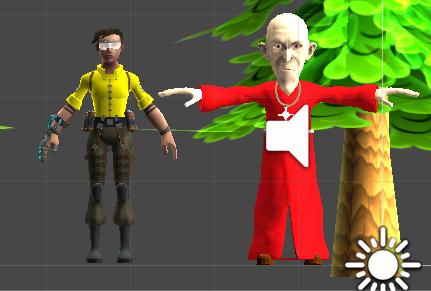
\includegraphics[width=0.6\textwidth]{img/both}
		\caption{Visual appearance of monk and darwinist.}
		\label{img:monkAndDarwinist}
	\end{figure}
	
	\newpage
	
	\begin{figure}[h!]
	\centering
	\begin{minipage}[t]{.5\textwidth}
	\centering
	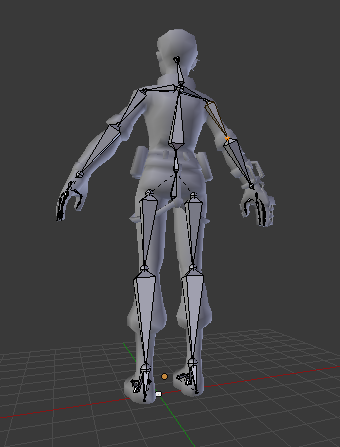
\includegraphics[width=0.7\textwidth]{img/engineer}
	\caption{Engineer back}
	\end{minipage}\hfill
	\begin{minipage}[t]{.5\textwidth}
	\centering
	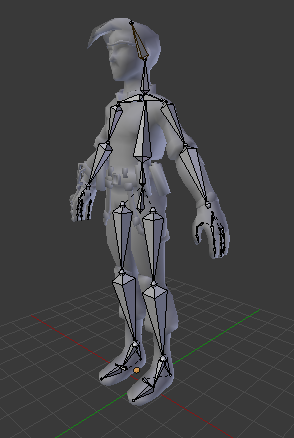
\includegraphics[width=0.7\textwidth]{img/engineer2}
	\caption{Engineer right side}
	\end{minipage}
	\end{figure}
	
	\begin{figure}[h!]
	\centering
	\begin{minipage}[t]{.3\textwidth}
	\centering
	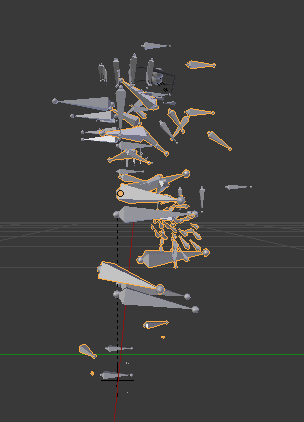
\includegraphics[width=0.7\textwidth]{img/skeleton-monk}
	\caption{Bones misplaced}
	\label{img:bones}
	\end{minipage}\hfill
	\begin{minipage}[t]{.3\textwidth}
	\centering
	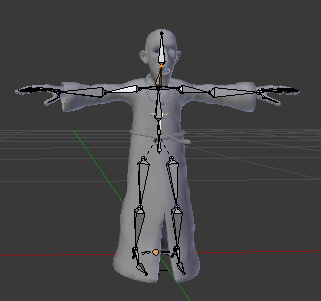
\includegraphics[width=1\textwidth]{img/monk1}
	\caption{Monk front}
	\end{minipage}
	\begin{minipage}[t]{.3\textwidth}
	\centering
	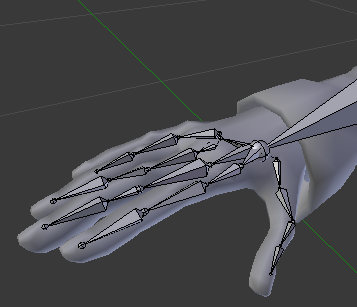
\includegraphics[width=1\textwidth]{img/monk2}
	\caption{Monk hand}
	\end{minipage}
	\end{figure}
	
	\newpage
	
	\subsection{Artificial Intelligence}
	
	\subsubsection{Clean Code}
	We realized quickly that the code responsible for the artificial intelligence (AI from here on) has to be well structured. When working and experimenting  with AI this code tends to get messy quickly. This is mainly due to the fact that, the AI needs to maintain a global structure of all Characters, their intentions and actions. Therefore, it does not suffice to handle a Collision in a local manner, but the action needs to be recorded and the strategy of the computer controlled players must be adapted accordingly. In addition, the decisions of the individual players must be explainable with the local knowledge of the individual player. \\
	
	\textbf{Solution: } Refactoring of previous code, sticking to coding conventions and maintaining an up to date and consistent structure of the game.
	
	\subsubsection{Performance}
	The algorithms executed by the non-human players have to be efficient. Since there can be many non-human players who are executing these procedures very often, we are restricted in their strategic complexity. It is for example unpractical to update the intention of each player in each step. This is, because potentially all players might influence each other player and thus, the number of pairs of players to consider were quadratic in the number of players. With increasing number of players this would not be feasible to compute in each step.\\
	
	\textbf{Solution: } The intentions of a player are only recomputed when a change makes sense. For example when a player is hit and hurled away he reorient himself. In addition, the exact movement is managed by each individual player, whereas the AI only decides on the intentions of the players (see Figure \ref{img:manyNPCs}).\\
	
	\begin{figure}[h!]
  		\centering
    	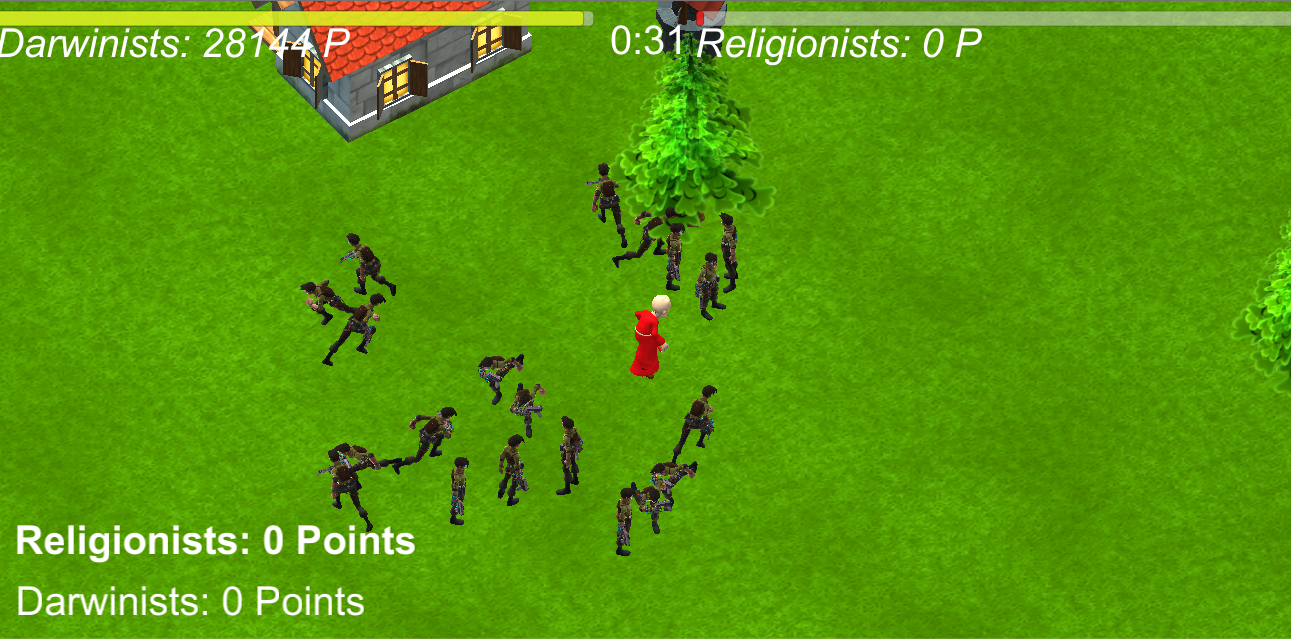
\includegraphics[width=0.6\textwidth]{img/scene2}
    	\caption{A player surrounded by a lot of non-human players controlled by AI}
    	\label{img:manyNPCs}
	\end{figure}
	
	\subsection{Game Logic}
	
	\subsubsection{People getting thrown off the map}
	When standing close to the edge of the map and being shot, it was possible to be hurled outside the map. Once this happened it was impossible to return to the map.\\
	
	\textbf{Solution: } See solution in Subsection \ref{subsubsection:wraparound} 
	
	
	\subsubsection{Wraparound Map}
	\label{subsubsection:wraparound}
	We wanted our map to be "Wrap-around". I.e. when you walk out on one side you would walk in on the opposite end of the map. This is necessary to prevent players from hiding in corners, where they cannot be thrown away when shot by an enemy. This would result in a massive advantage when praying or studying because the group cannot be scattered by shooting inside it. Maps with a wrap-around are not natively supported by Unity. Thus, we would have to implement it which would become extremely complicated in terms of many objects which would have to be relocated and reinstantiated at any moment. We would not be able to use solely the physic engine's procedures like for example collision checks, if they would happen in a wrap-around scenario.
	
	\textbf{Solution: } We implemented the map as a island with surrounding water. As soon as a player falls into the water he is respawned somewhere on the map.	
	
	\begin{figure}[h!]
  		\centering
    	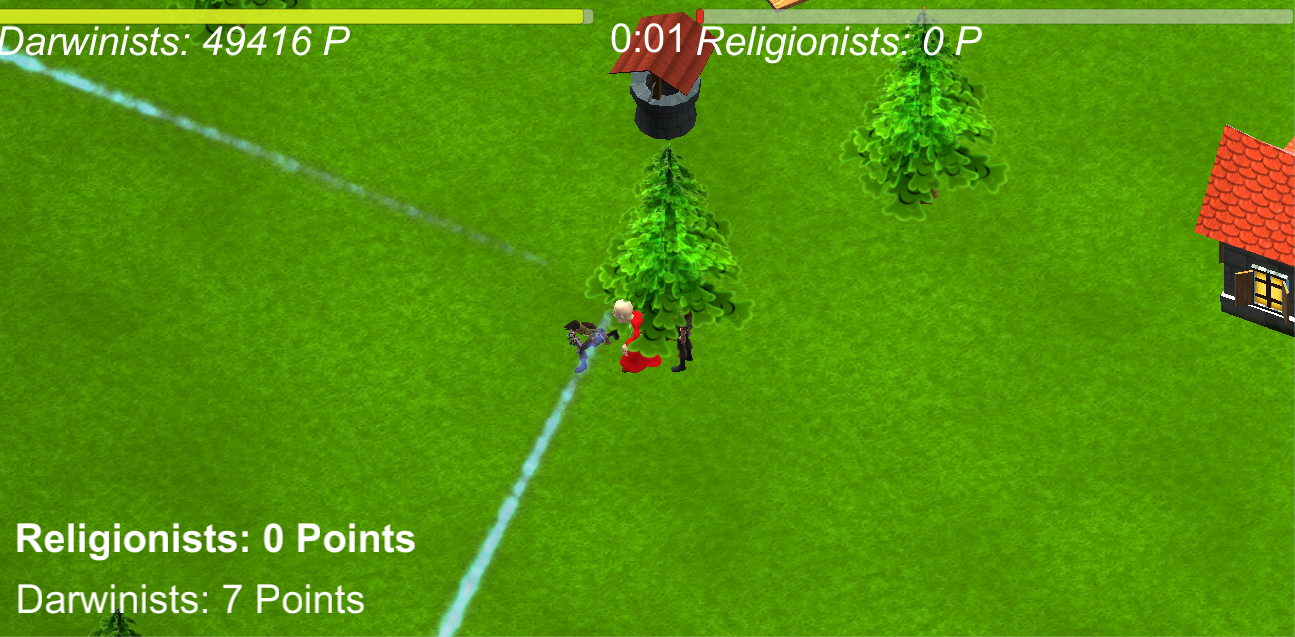
\includegraphics[width=0.6\textwidth]{img/in-tree}
    	\caption{A player being attacked while standing within a tree}
    	\label{img:spawnwithinobject}
	\end{figure}
	
	\subsubsection{Spawning Points}
	Initially we generated random spawning points. However, sometimes this lead to a scenario where a player would spawn inside some other element, for example a house or a tree. Such a player was not able to get outside of the element and could only shoot from its stationary position (see Figure \ref{img:spawnwithinobject}).\\
	\textbf{Solution: } Ask the NavMesh whether the random position is free and on the map.

	\section{Interim Conclusion}
	We are well on our way to make this a fun game and while we have had to tackle a few obstacles already we have not run into an issue that would cause us to make severe game design changes.

	
\end{document}}{den}
